\documentclass[tikz,border=15pt]{standalone}
\usepackage{tikz}
\usetikzlibrary{arrows.meta, positioning, fit, patterns}

\begin{document}

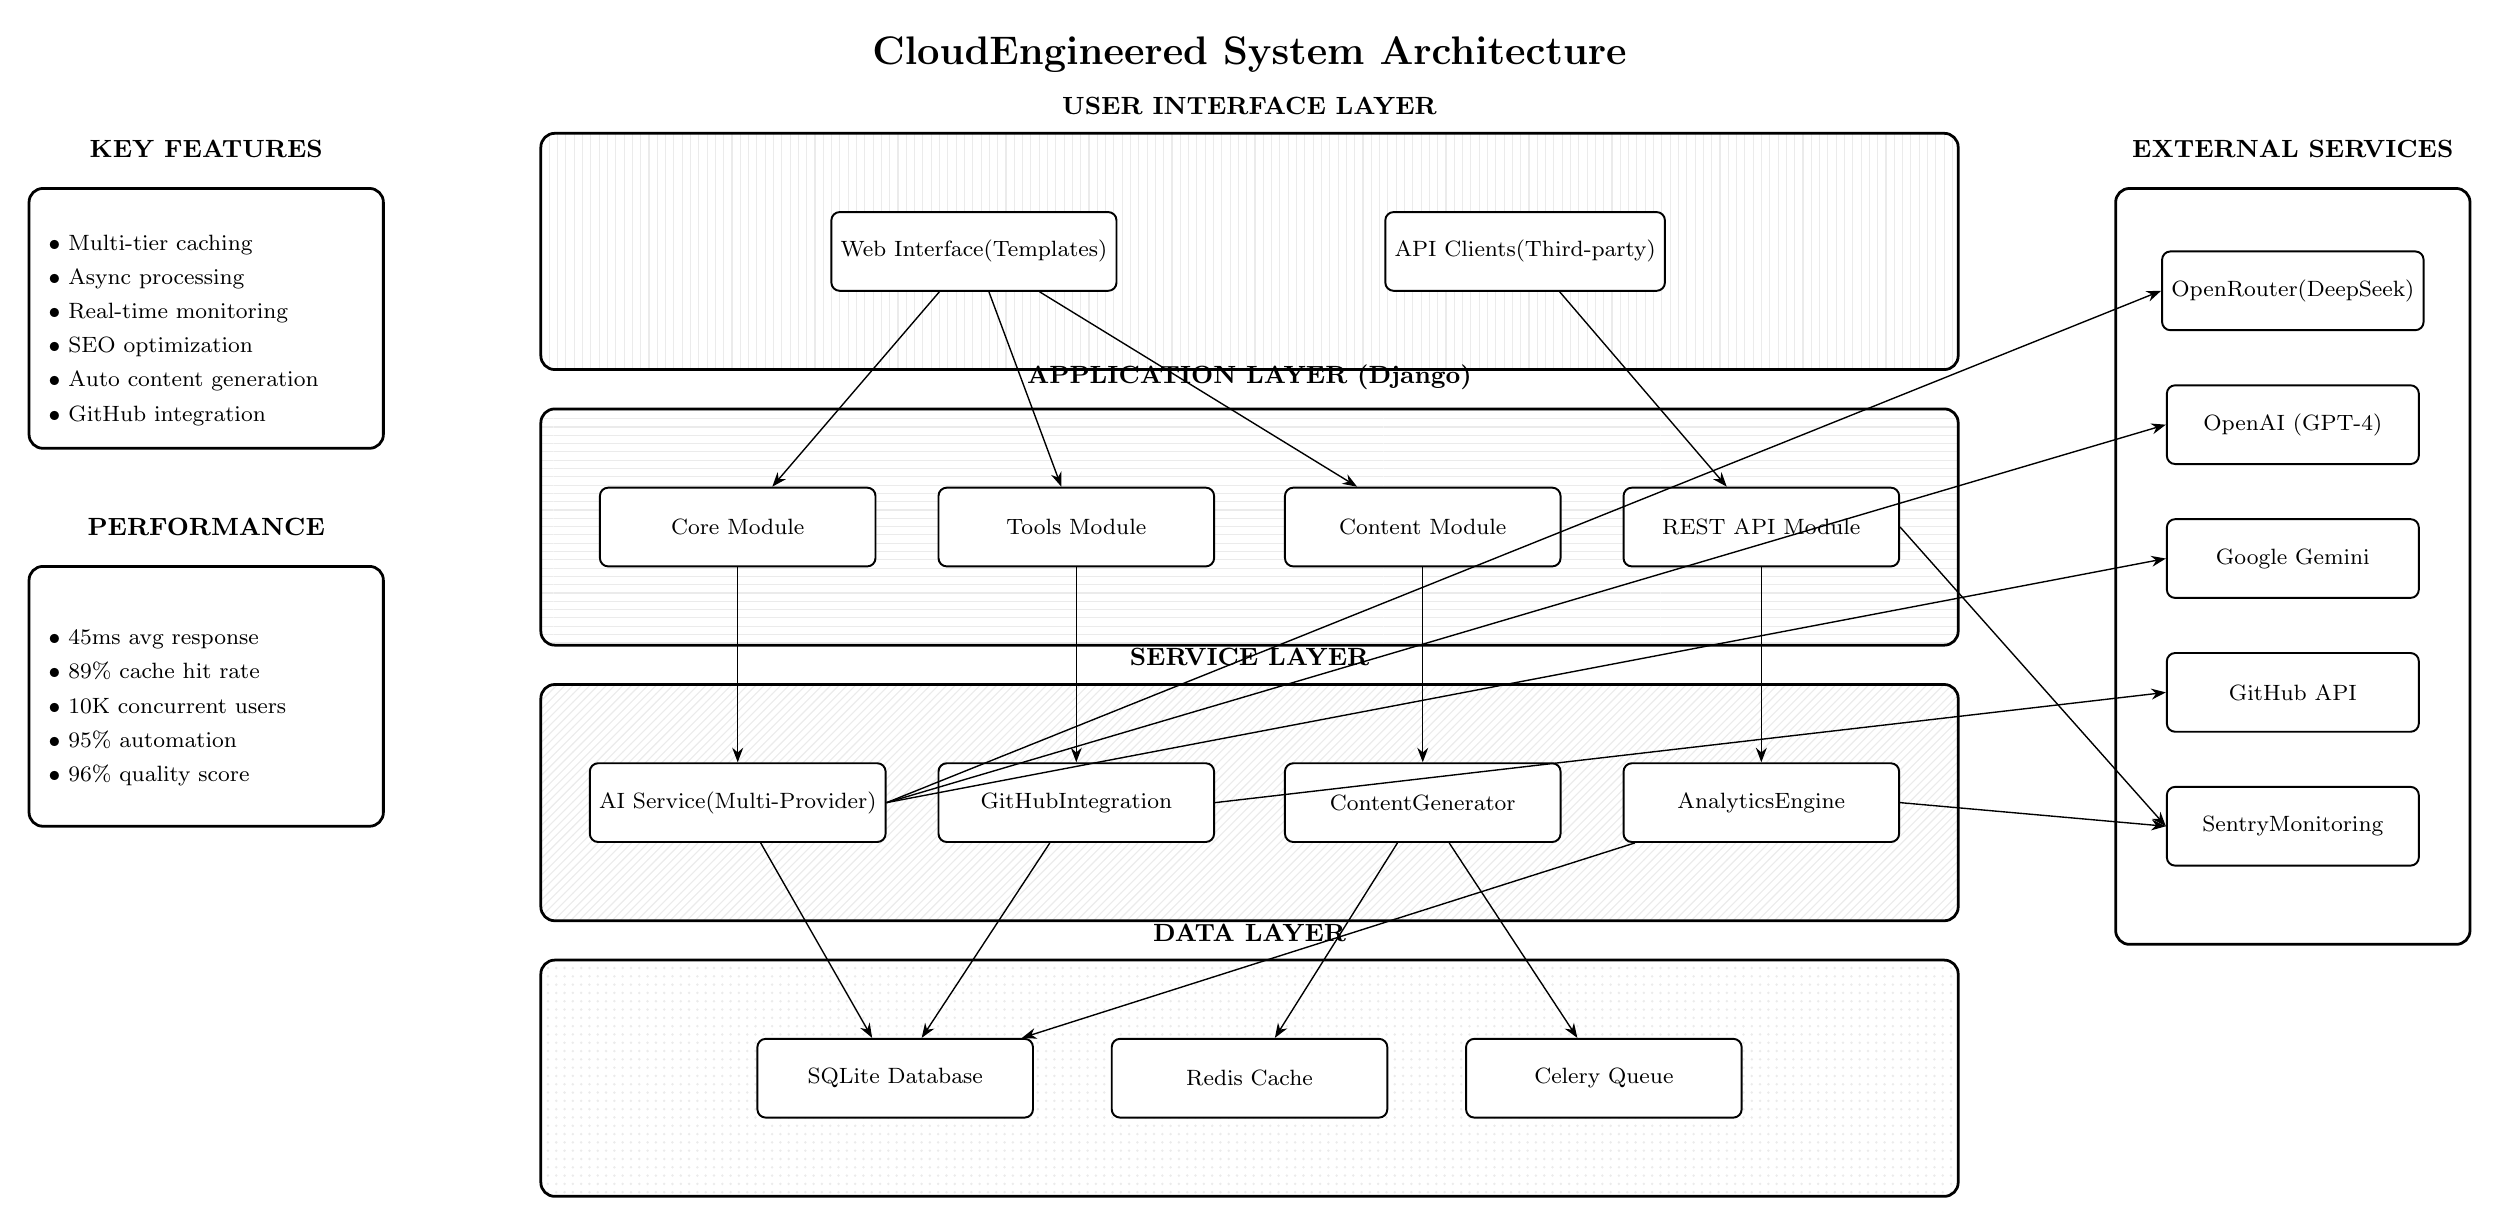
\begin{tikzpicture}[
    node distance=1.5cm and 1cm,
    box/.style={rectangle, rounded corners=3pt, minimum width=3.5cm, minimum height=1cm, 
                text centered, draw=black, line width=0.7pt, fill=white, font=\footnotesize},
    layerbox/.style={rectangle, rounded corners=5pt, minimum width=18cm, minimum height=3cm, 
                     draw=black, line width=1pt, fill=white},
    arrow/.style={->,>=Stealth,line width=0.5pt},
    labelstyle/.style={font=\small\bfseries}
]

% Title
\node[font=\Large\bfseries] at (0, 16.5) {CloudEngineered System Architecture};

% ==================== LAYER 1: USER INTERFACE ====================
\node[layerbox, pattern=vertical lines, pattern color=black!8] (ui-layer) at (0, 14) {};
\node[labelstyle, above=0.1cm of ui-layer.north] {USER INTERFACE LAYER};

\node[box] (web-ui) at (-3.5, 14) {Web Interface\\(Templates)};
\node[box] (api-clients) at (3.5, 14) {API Clients\\(Third-party)};

% ==================== LAYER 2: APPLICATION ====================
\node[layerbox, pattern=horizontal lines, pattern color=black!8] (app-layer) at (0, 10.5) {};
\node[labelstyle, above=0.1cm of app-layer.north] {APPLICATION LAYER (Django)};

\node[box] (core) at (-6.5, 10.5) {Core Module};
\node[box] (tools) at (-2.2, 10.5) {Tools Module};
\node[box] (content) at (2.2, 10.5) {Content Module};
\node[box] (api) at (6.5, 10.5) {REST API Module};

% ==================== LAYER 3: SERVICE ====================
\node[layerbox, pattern=north east lines, pattern color=black!8] (service-layer) at (0, 7) {};
\node[labelstyle, above=0.1cm of service-layer.north] {SERVICE LAYER};

\node[box] (ai-service) at (-6.5, 7) {AI Service\\(Multi-Provider)};
\node[box] (github-service) at (-2.2, 7) {GitHub\\Integration};
\node[box] (content-service) at (2.2, 7) {Content\\Generator};
\node[box] (analytics-service) at (6.5, 7) {Analytics\\Engine};

% ==================== LAYER 4: DATA ====================
\node[layerbox, pattern=dots, pattern color=black!8] (data-layer) at (0, 3.5) {};
\node[labelstyle, above=0.1cm of data-layer.north] {DATA LAYER};

\node[box] (database) at (-4.5, 3.5) {SQLite Database};
\node[box] (cache) at (0, 3.5) {Redis Cache};
\node[box] (celery-broker) at (4.5, 3.5) {Celery Queue};

% ==================== EXTERNAL SERVICES ====================
\draw[line width=1pt, rounded corners=5pt] (11, 14.8) rectangle (15.5, 5.2);
\node[labelstyle] at (13.25, 15.3) {EXTERNAL SERVICES};

\node[box, minimum width=3.2cm] (openrouter) at (13.25, 13.5) {OpenRouter\\(DeepSeek)};
\node[box, minimum width=3.2cm] (openai) at (13.25, 11.8) {OpenAI (GPT-4)};
\node[box, minimum width=3.2cm] (gemini) at (13.25, 10.1) {Google Gemini};
\node[box, minimum width=3.2cm] (github-api) at (13.25, 8.4) {GitHub API};
\node[box, minimum width=3.2cm] (sentry) at (13.25, 6.7) {Sentry\\Monitoring};

% ==================== INFO BOXES ====================
\draw[line width=1pt, rounded corners=5pt] (-15.5, 14.8) rectangle (-11, 11.5);
\node[labelstyle] at (-13.25, 15.3) {KEY FEATURES};
\node[align=left, font=\footnotesize, text width=4cm] at (-13.25, 13) {
    $\bullet$ Multi-tier caching\\[0.1cm]
    $\bullet$ Async processing\\[0.1cm]
    $\bullet$ Real-time monitoring\\[0.1cm]
    $\bullet$ SEO optimization\\[0.1cm]
    $\bullet$ Auto content generation\\[0.1cm]
    $\bullet$ GitHub integration
};

\draw[line width=1pt, rounded corners=5pt] (-15.5, 10) rectangle (-11, 6.7);
\node[labelstyle] at (-13.25, 10.5) {PERFORMANCE};
\node[align=left, font=\footnotesize, text width=4cm] at (-13.25, 8.2) {
    $\bullet$ 45ms avg response\\[0.1cm]
    $\bullet$ 89\% cache hit rate\\[0.1cm]
    $\bullet$ 10K concurrent users\\[0.1cm]
    $\bullet$ 95\% automation\\[0.1cm]
    $\bullet$ 96\% quality score
};

% ==================== ARROWS ====================
% UI to Application
\draw[arrow] (web-ui) -- (core);
\draw[arrow] (web-ui) -- (tools);
\draw[arrow] (web-ui) -- (content);
\draw[arrow] (api-clients) -- (api);

% Application to Service
\draw[arrow] (core) -- (ai-service);
\draw[arrow] (tools) -- (github-service);
\draw[arrow] (content) -- (content-service);
\draw[arrow] (api) -- (analytics-service);

% Service to Data
\draw[arrow] (ai-service) -- (database);
\draw[arrow] (github-service) -- (database);
\draw[arrow] (content-service) -- (cache);
\draw[arrow] (analytics-service) -- (database);
\draw[arrow] (content-service) -- (celery-broker);

% External Services
\draw[arrow] (ai-service.east) -- (openrouter.west);
\draw[arrow] (ai-service.east) -- (openai.west);
\draw[arrow] (ai-service.east) -- (gemini.west);
\draw[arrow] (github-service.east) -- (github-api.west);
\draw[arrow] (analytics-service.east) -- (sentry.west);
\draw[arrow] (api.east) -- (sentry.west);

\end{tikzpicture}

\end{document}
